\section{Detector layout}
\subsection{The EM calorimeter (FT-Cal)}

The FT-Cal has to  fulfill demanding requirements in terms of:  radiation hardness, light yield, shower containment (small radiation length and Moliere radius), fast recovery time, good energy and time resolution.

The electron energy resolution is a crucial factor to determine precisely the photon energy and ensure the exclusivity of the measured reaction via missing mass technique. However, since we are interested in low energy electrons and high energy photons, the energy resolution on the latter is significantly better than the resolution on the electron
\footnote {For example, an electron energy resolution of 2\% (at 1 GeV) would result in an energy resolution of $\sim 0.2 \%$ for the corresponding 10 GeV photon allowing  the use the missing mass technique for the most part of the  reactions of iterest.}.  
The FT-Cal should  have a fast recovery time ($\tau\sim$ 10 ns) to sustain high rates with small pile-up effects and provide the scattered electron interaction time with good accuracy ($<$1 ns) in order to reject background and identify the signal via coincidence with CLAS12. Due to the expected high rate from electromagnetic background, the calorimeter should be highly segmented in the transverse direction. The size of each pixel
should be comparable with the characteristic transverse size of the electromagnetic shower (Moliere radius) to contain the  shower produced  by incident electrons to few pixels, thus minimizing the pixel rates and pile-up. 
Finally, the photodetectors for the light read-out should work  in a sizable magnetic field and has to be small in size to fit within the available space. Thus, the  standard photomultipliers can not be used  while photodetectors based on semiconductors, e.g. Avalanche Photo Diode (APD),   have been shown to meet the required criteria. 

To match the necessary requirements,  PbWO$_4$  was chosen as scintillating material and  {\it Large-Area} APDs (LAAPD) as readout sensors. A similar  combination was used in CMS-ECal~\cite{CMS}, CLAS-IC~\cite{ic} and PANDA-EMC~\cite{panda_ecal}. Lead-tungstate has a fast scintillation decay time (6.5 ns), a  small radiation length (0.9 cm) and  small Moliere radius (2.1 cm). The drawback of  limited light emission (about 0.3\% of NaI(Tl)) has been mitigated by using cooled PbWO Type-II crystals (as PANDA-ECAL) matched  to large area photo sensors obtaining a x4 more light per MeV than the original CMS ECal crystals.

With this design
 an energy resolution of \\
($2\% /\sqrt{E(GeV)} \oplus 1\%$) is expected.
Other crystals as LSO/LYSO (or the very recent LaBr) share almost all the good specifications of the PbWO$_4$ with a light yield more than 100 times bigger. However, the lack of extensive studies on radiation hardness and limited experience in the manufacturing procedures prevented them to be considered as an alternative.

\begin{figure}[th!]
\centering 
%\includegraphics[width=0.85\columnwidth]{fig/ft-cal-geometry.pdf} 
\caption{} 
\label{fig:ft-cal-geometry} 
\end{figure}

\subsubsection{Geometry and coverage}
The FT-Cal is made by 332 15x15x200 cm$^3$ parallelepiped PbWO$_4$ Type-II crystals arranged around the beam line  with full azimuth angular coverage ($0^o<\phi<360^o$)   and small forward angles  acceptance ($2^o<\theta<5^o$). Crystals are placed with the long side parallel to the beam line to form a ring. Figure~\ref{fig:ft-cal-geometry} shows the crystal assembly. 

\subsubsection{PbWO$_4$ crystals}
FT-Cal PbWO$_4$ Type-II crystals were produced by the Shanghai Institute of Ceramics, Chinese Academy (SICCAS). Since the light yield (LY) increases while lowering the temperature T according to $dLY/dT \sim 3\%/^oC$, the calorimeter is stabilized in temperature and operated at T$\sim 0 ^oC$. Lower T were not considered due to a significant complication in the mechanical/thermal design,  the reduced resistance to radiation  and the decay time degradation showed by cooled PbWO$_4$.
The length of the crystal (20 cm corresponding to $\sim22$ EM radiation lengths) was chosen to minimize the longitudinal loss matching the available clearance.

The face lateral size of 15mm x 15mm  provides the highest pixelization in the transverse plane being  of the same size of  PbWO$_4$  Moliere radius.  All crystals were characterized using the ACCOS (Automatic Crystal quality Control System) facility  at CERN \cite{accos}. Geometrical dimensions as well as optical properties such as longitudinal and transverse  transmission and relative light yield were determined for each crystals. Samples out of the required specifications were rejected and replaced by the manufacturer. 

The absolute LY (number of detected phto-electron per MeV deposited) was found to be N$_{pe}$=220$\pm$20 at T=$0^o C\pm 0.5C^o$. For this measurement  the crystal was wrapped on 5 faces with 3M Vikuiti reflective film \cite{vm2000} and light read by a Large Area APD Hamamatsu S8664-1010 operated at a G=150 connected with optical grease on the free side. 

The scintillation decay time is also sensitive to the temperature. The time constant was measured using the {\it Start-Stop} or {\it delayed coincidence} method at different T. As expected an increase in the decay constant was observed by decreasing the temperature. At T=$0^oC\pm 0.5C^o$ we found $\tau=13.5\pm 0.6$ ns ($\tau_1=11.6\pm 0.5$ ns and $\tau_1=13.0\pm 0.2$ ns) when a single (double) exponential form was used to fit the data.



\begin{figure}[th!]
\centering 
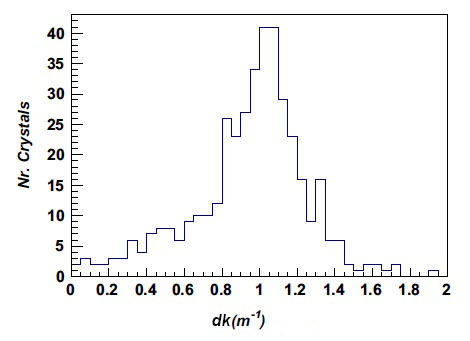
\includegraphics[width=0.85\columnwidth]{./fig/dk.jpeg} 
\caption{Histogram of the radiation induced absorption coefficient, dk, for all SICCAS FT-Cal
 PbWO$_4$ crystals.}
\label{fig:dk} 
\end{figure}
The radiation hardness of the crystals was measured  by irradiating crystals with a dose of 30 Gy of  low energy photons using a $^60$Co source at the Strahlenzentrum of Giessen University \cite{radhard}. The longitudinal transmission was measured before and after the irradiation calculating the variation as a function of the light-wave length. Radiation hardness of the crystals is quantified by the radiation induced absorption coefficient defined as:
\begin{equation}
dk = \frac{1}{length}\frac{T_{bef}}{T_{irr}}
\end{equation}
where $T_{bef}$ is the light transmission at 420 nm, the peak of the PbWO$_4$ emission spectrum, measured before irradiation, and $T_{irr}$ the light transmission at the same wave-length  after irradiation. 
Crystals exhibiting greater levels of radiation damage to light transmission have higher values of $dk$. 
All 332 crystals assembled in the FT-Cal were individually characterized: on average we found 
$T_{bef}(420 nm) = 61.5 \pm 0.2$ ($\sigma=3.2$) and 
$T_{irr}(420 nm) = 50.8 \pm 0.5$ ($\sigma=4.9$). 
The resulting $dk$ distribution is shown in Fig.~\ref{fig:dk}.
These measurements were used to optimize the position of each crystal in the calorimeter, placing the crystals with the highest radiation resistance and therefore lowest $dk$ in the areas where the highest radiation dose is expected.

\begin{figure}[th!]
\centering 
\includegraphics[width=1.0\columnwidth]{./fig/apd5.eps} 
\caption{Intrinsic gain of one APD as a function
of the bias voltage and of the temperature.}
\label{fig:G-V-T} 
\end{figure}

\subsubsection{Light readout and electronics }
The FT-Cal uses 10x10 mm$^2$ (model Hamamatsu S8664-1010) Large Area Avalache Photo Diodes (LAAPDs) to read out the scintillation light. APDs are very compact devices (only few mm thick),  have a large quantum efficiency at the PbWO$_4$ light peak emission (420 nm), and  are insensitive to magnetic fields. The main disadvantage is that, due to
the low intrinsic gain ($\sim 50-200)$, the output signal is too small to be directly acquired, and needs to be amplified
by a suitable circuit. APDs also need
to be operated at controlled temperature to
avoid variations in gain and noise but this does not represent a major complication since the crystals too require to be stabilized in temperature.
Each sensor used in the FT-Cal has been characterized by measuring the gain as a function of the applied bias voltage at a given temperature using an automated  custom facility (see Ref.~\cite{celeAPD} for more details). The typical behaviour G(V$_{Bias}$,T) is shown in Fig.~\ref{fig:G-V-T}.The working point (bias voltage) was chosen in order to have the chosen gain (G=150) still laying in a reasonably stable region for small variation of the biasing. SiPM readout was not considered due to their limited dynamical range not suitable for spectroscopic application and the limited experience (in term of reliability, radiation hardness, stability in time, ...) in their use in large experiments at the time.\\

%Electronics

The APD current signal is converted to a
voltage pulse which is transmitted to the subsequent
electronics chain via a trans-impedance
amplifier (i.e. an amplifier which converts an
input current pulse into an output voltage
pulse, without performing any time integration).
This amplifier has been developed in
collaboration with the “Service d’Electronique
Physique” (SEP) of the “Institut de Physique
Nucleaire” (IPN) in Orsay. The amplifier ENC \footnote{The ENC, “equivalent noise charge” is defined as the
charge transported by that input signal giving, at the
output of the amplifier, a signal whose amplitude is equal
to the RMS of the output noise.} was measured at the operation temperature (T=0$^o$ C,  finding ENC=(8200$\pm$100) e$^-$ (rms) for the nominal gain of G=1800 (CORRECT TO ACCOUNT THE FINAL GAIN WAS SET TO 600). 
The amplified signal is read using the custom JLab fADC  250 board (a 16ch, 12 bit, 250 MHz, VME digitizer extensively used at JLab). The measurement of the full wave form allows to derive both charge and time of the hit with the required   accuracy.

\subsubsection{Light Monitoring System}
% Light Monitoring
Lead tungstate scintillating crystals are known
as an appropriate material for use in total absorption
shower detectors. Unfortunately, although
relatively radiation tolerant, they do
lower their light output when exposed to radiation
and recover when the radiation source is
removed. Further complications
arise because at the same irradiation intensity, changes in light output may vary from
one crystal to another.
In order to maintain the intrinsic energy resolution, crystals
have to be continuously monitored and
if necessary, re-calibrated changing the supply voltage.
The monitoring system should be able to 
 test over the time  the response of the whole chain: crystal,
APD, red-out electronics.
Among the different possible options (radioactive source, laser and LED) we used an LED base Light Monitoring System (LMS). In spite of the
need of a thermal control, LEDs offer
considerable advantages: matching with
crystals is more simple than for lasers,
since each crystal can have a LED in
front of it and the arrangement of electric
wires is less critical than optical fibers.
The main disadvantage is related to the
complexity of the electric circuitry: to
cover a large light range keeping a good
timing, each LED needs a separate driver
leading, for calorimeter of significant size,
to a large number of electronic circuits.
With LEDs it is
possible to obtain a shape and a duration
of the monitoring-light flash that would be
similar to the features of the crystal scintillation.
In fact: the emission spectrum of
the monitoring light can be chosen similar to
the radio-luminescence spectrum of PbWO$_4$,
the effective optical path length for monitoring
light in the crystal can be matched to
the average path length of the scintillation
light produced by an electromagnetic shower,
and pulse length can be tuned to reproduce
the PbWO$_4$ scintillation decay time. We chose a blue light LED with wavelength close to the 430 nm emission
peak of the PbWO$_4$ crystal and where the
radiation damage may have the maximum effect.
Each crystal is equipped with a separate LED, located on
the upstream face of each crystal, at the
opposite end respect to the light sensors
and electronics. Intensity can be varied in
a range from 500 to 100.000 photons, pulsed at  variable rate between 62 Hz to 8 kHz, with pulse rise time of $\sim1$ ns and a time jitter less than 200 ps. The system has been 
designed to work in the temperature range -25 $^o$C +30 
$^o$C. LEDs, placed in the closed
environment of the crystal,is kept at
constant temperature with an accuracy of $\Delta T$ =
0.1$^o$C. The LED monitoring system is split in two
boards: one containing the control logic and
the LED driver circuits, and the other, to be
mounted in front of the FT-Cal crystals, hosting
the LEDs. The two boards are connected
via a board-to-board connector allowing the
required flexibility to match the FT-Cal geometry
and positioning. The LED drivers are controlled by an on-board PIC32 micro-controller accessible remotely  via Ethernet.
\begin{figure}[th!]
\centering 
\includegraphics[width=1.0\columnwidth]{./fig/dynamics.eps}
\caption{Number of photoelectrons as a function
of the driver current. The corresponding energy
per crystals range form 10 MeV to 10 GeV.}
\label{fig:LEDperf1} 
\end{figure}
\begin{figure}[th!]
\centering 
\includegraphics[width=1.0\columnwidth]{./fig/timing.eps}
\caption{Time resolution measured as the difference of trigger signal and the PMT pulse.}
\label{fig:LEDperf2} 
\end{figure}
Each LED is individually lighted by a programmable
lenght and intensity pulse. The
system is triggered by an internal clock or by
an external signal. In both cases the trigger
signal is available for a precise time reference.
The performance of the LED driver
has been measured coupling a single monitoring
channel to a photomultiplier. Performance of the system are reported in Figs.~\ref{fig:LEDperf1} and ~\ref{fig:LEDperf2} where the measured photoelectrons
as a function of the led current and the measured time resolution as
a function of the number of photoelectron are shown\footnote{Time resolution is defined as the sigma of the time difference distribution
between the trigger signal and the
PMT output.}. Rescaling
results to take into account the APD readout
and the crystal LY/MeV the equivalent
energy ranges from 10 MeV (500 phe) to 10
GeV (500k phe) perfectly matched to the expected
energy collected by each crystal. A time resolution
of 100 ps is reached at high light
intensity. Long term stability of the system has been measured and over 100h (4 days) run at
T=+18 $^o$C, a stability of each individual
channel has been found to be in the range of 2$\%$;  when the ratio
of the two channels is considered,
the stability is at level of few $\textperthousand$.
%Figure~\ref{fig:LED-assembly} shows the FT-CAL LSM.

\subsubsection{Slow controls}
The FT-Cal slow controls are part of the CLAS12 EPICS system (see Sec.~\ref{sec:slowcontrols}.
APD  needs to be reverse-biased
with an high-voltage positive power
source. The APD intrinsic
gain depends on the bias voltage with
$\frac{1}{G}\frac{\Delta G}{\Delta V} \sim4 \%$
and therefore the power supply
needs to be stable in time, with low output
noise. We chose the CAEN board A1520P designed
for the CMS electromagnetic
calorimeter. The power supply fulfills  all our requirements in
terms of dynamic range, linearity and noise.
Each board is equipped with 12 independent
channels each of them controlling a group of ten APDs
 with relative
gain variations not greater than 3$\%$.

The amplifiers used in the FT-Cal need to
be operated with +5 V and -5 V.
The power consumption from
each of the two voltage sources is approximately
70 mW, almost independent on the
event rate, giving a power consumption of
$\sim$140 mW per board, for a total of 56 W for
a 400-channels calorimeter. 
The full FT-Cal is powered by a Wiener
{\it MPOD universal low voltage power supply} MPV8008L,
the same module used for other CLAS12 low voltages.
Sensing is implemented
to compensate the voltage drop across
the connecting cables.

Temperature regulation is provided by a
Lauda XT150 chiller unit. This is a self regulating
unit and does not require external feedback;
however the settings and monitored parameters are sent to EPICS for recording via a
{\it streamDevice} module.
The FT-Cal temperature is 
 monitored by a set of PT100 thermoresistors.
read by a {\it cRio} module which is being used in the other CLAS12 subsystems, which is part of the interlock system~\ref{sec:interlocks}.

\subsubsection{Mechanical design}
The mechanical design of the calorimeter is
driven by three considerations: minimization of the empty spaces between
crystals, cooling to 0 $^O$C; optimal coverage of the requested acceptance without interference with the rest
of CLAS12.
\begin{figure}[th!]
\centering 

\includegraphics[width=1.0\columnwidth]{./fig/sc-assembly.eps}
\caption{Single crystal assembly: from the
left (front) to the right (back), the PEEK holding nose with the LED housing, the
crystal wrapped in 3M Vikuiti reflective film, the LAAPD in the PEEK housing, and
the  preamplifier.}
\label{fig:crystalassembly} 
\end{figure}

The building block of the calorimeter is the
single lead-tungstate crystal. Each crystal
is 15x15x200 mm$^3$, for a weight of
370 g.
Each crystal is optically coupled
to a Large Area APD on back side  and to an LMS LED on the front side for calibration. To achieve the maximum
light collection efficiency, the APD covers
almost the whole area of the downstream
end of the crystal, so the LED for monitoring
will be hosted on the upstream end. This
reflects onto the mechanical design of the single
crystal assembly 
as a monolithic self-supporting element made of
the crystal itself, the APD, the reflective coating
 and some support structure.
To avoid dead volume in the detector,
the mechanical support for each crystal is provided only by wrapping. We chose 3M Vikuiti reflective film. This material is non conductive, has a reflectivity higher
than aluminized Mylar and, if properly
hot-formed, can hold the weight of a crystal. The reflective film is glued on the sides of a pair of front/back PEEK custom-machines blocks that hold the LAAPD and the LED, respectively. Figure~\ref{fig:crystalassembly} shows the CAD rendering of the single
crystal assembly from the frontal PEEK support
to the  preamplifier.
\begin{figure}[th!]
\centering 
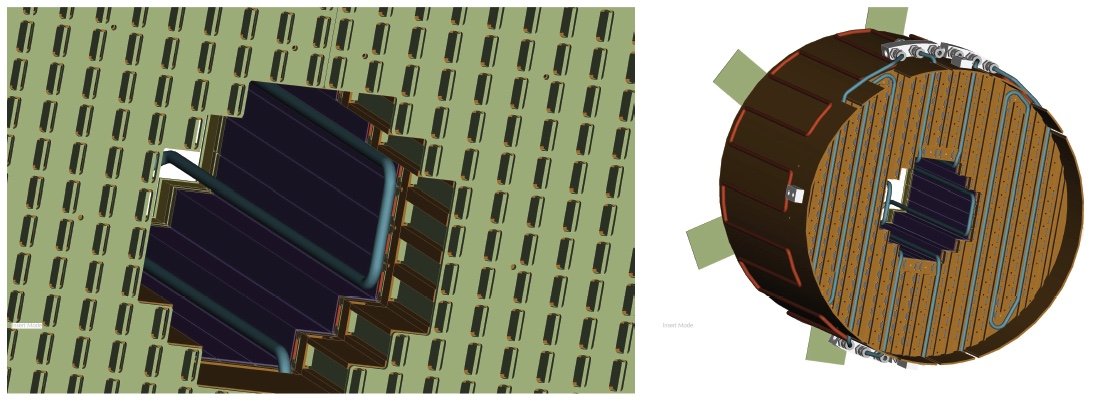
\includegraphics[width=1.0\columnwidth]{./fig/raff.jpeg}
\caption{The copper thermal/grounding shield
with the cooling pipes.}
\label{fig:piping} 
\end{figure}

The crystal assemblies are installed in an
matrix to provide complete shower containment
for electrons in the FT-Cal angular acceptance.
Two copper plates, placed in front and on the back of the crystals, provides load path
and positioning for the crystal assemblies. On
the APDs side, the preamplifiers, one for each crystal, are connected to the mother board PCB, which is designed to provide power supply, HV distribution and signal collection for
each channel. The mechanical structure allows one to 
to replace individual preamplifiers if needed. The front and back copper plates are connected by a copper cylindrical calendar on the outside and by an inner copper shield to form a closed vessel surrounding the crystal matrix to provide proper grounding and the required thermal stability and uniformity. Cooling is provided by 5-mm diameter copper pipes installed on the outside of the vessel as shown by  Fig~\ref{fig:piping}. A CAD section
view of the complete calorimeter is shown in Fig~\ref{fig:calsec}.
\begin{figure}[th!]
\centering 
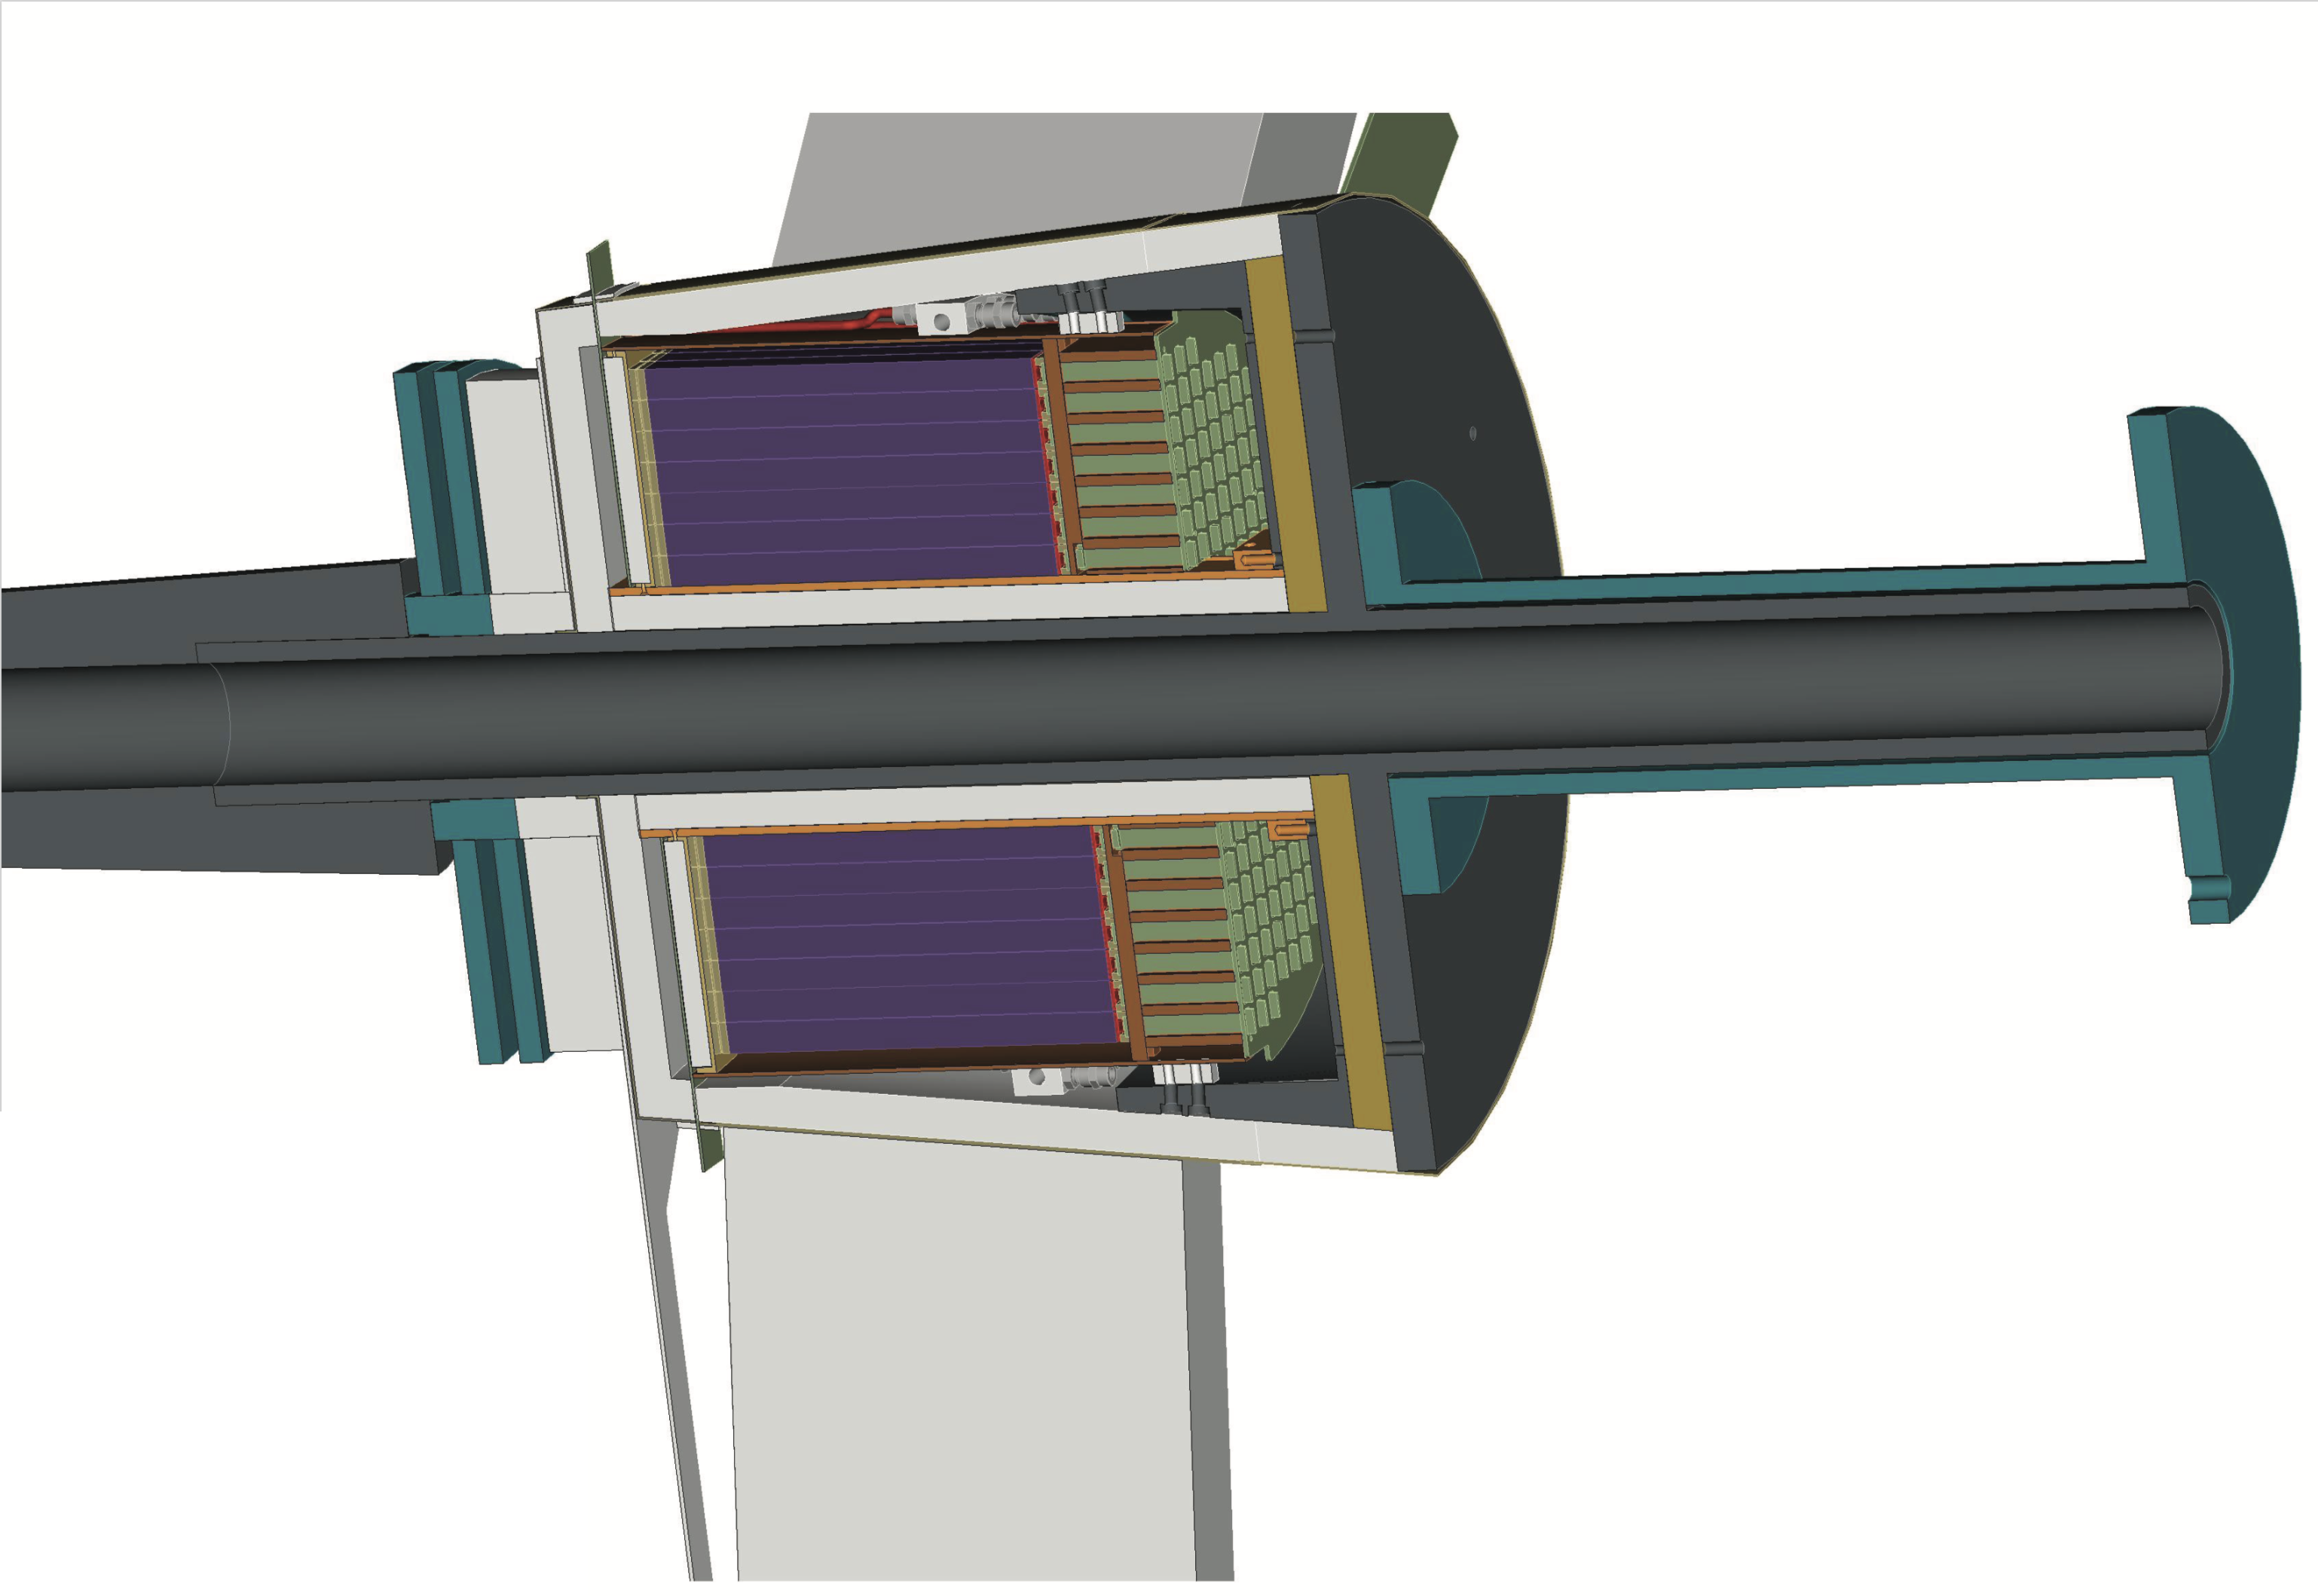
\includegraphics[width=1.0\columnwidth]{./fig/section.eps}
\caption{Cross section of the FT calorimeter: in purple, the crystals, upstream the PEEK forward blocks and the forward copper plate, downstream the rear copper plate, the preamplifiers (in green) and the mother board (in white), in light blue and yellow, part of the insulation.}
\label{fig:calsec} 
\end{figure}


The FT calorimeter has been designed to operate
between 0$^o$C to room temperature. FT-Cal cooling  is achieved via circulation
of coolant in the circuit attached to the rear copper
plate and on the inner and outer copper
vessels. The cooling system has been designed
to compensate the heat inlet coming
from the outside world, taking into account
20 mm of insulating foam (Polyisocianurate,
declared thermal conductivity 0:024W/mK)
and from the amplifiers, which  dissipate $\sim$50 W.
The insulation is less effective between the
calorimeter and the inner tungsten pipe that holds the entire FT (see Sec.~\ref{sec:integration}), because of the limited space for the insulation and the presence of support structures that bring the overall thermal conductance in that region to
0.056W/mK.

During the design phase, Finite Elements calculation 
were performed to optimize the cooling circuit and insulation parameters in order to reach the 
design temperature and
uniformity. These studies indicated that the coldest part of the external calorimeter enclosure is 
the tungsten cone that is expected to stabilize
at a temperature just above than the dew
point. Measurements performed after the calorimeter assembly confirmed these results.


\subsection{The hodoscope (FT-Hodo)}
The primary aim of the FT-Hodo is to discriminate between photons and electrons that produce the electromagnetic shower in the calorimeter. Specifically, electrons are identified by hits in the hodoscope array which are correlated in both position and time with a cluster observed in the calorimeter. The FT-Hodo comprises an array of 232 plastic scintillator (Eljen-204) tiles segmented in two layers to suppress contributions from the splash-back of the electromagnetic shower created by events depositing energy in the FT-Cal. The scintillators provide fast timing and sufficient resistance to radiation damage for use in the high rate and high dose environment of the Forward Tagger. The geometry and readout of the hodoscope are constrained by the surrounding apparatus. Specifically, the device is positioned upstream of the FT-Cal fitting into a circular disk of diameter 330~mm and 42~mm depth. The readout is achieved using $3\times 3$~mm$^2$ Hamamatsu S13360-3075PE SiPMs (50\% photon detection efficiency for 450~nm photons) coupled to 5~m long clear optical fibres (Kuraray clear-PSM with attenuation length $>10$~m), which are fusion spliced to $\sim 30~$cm long wavelength shifting (WLS) Kuraray Y11 fibres (attenuation length of $> 3.5$~m), embedded in the scintillator tiles. The splicing induces a photon loss of less than 2\%, where the use of optical fibres allows the captured light to be transported with a light loss less than $\sim40\%$ over the 5 meter path to the SiPM. This readout design of the FT-Hodo addresses the need to minimise material in the detector acceptance, to operate in regions of high magnetic fields produced by the CLAS12 solenoid and torus magnets, and to tolerate the high background radiation environment. 


Each layer of the FT-Hodo comprises of 44 $15\times 15$~mm (P15) and 72 $30\times 30$~mm (P30) scintillators arranged as shown in Fig.~\ref{Fig:FTHodoLayout}  
\begin{figure}[th!]
\centering 
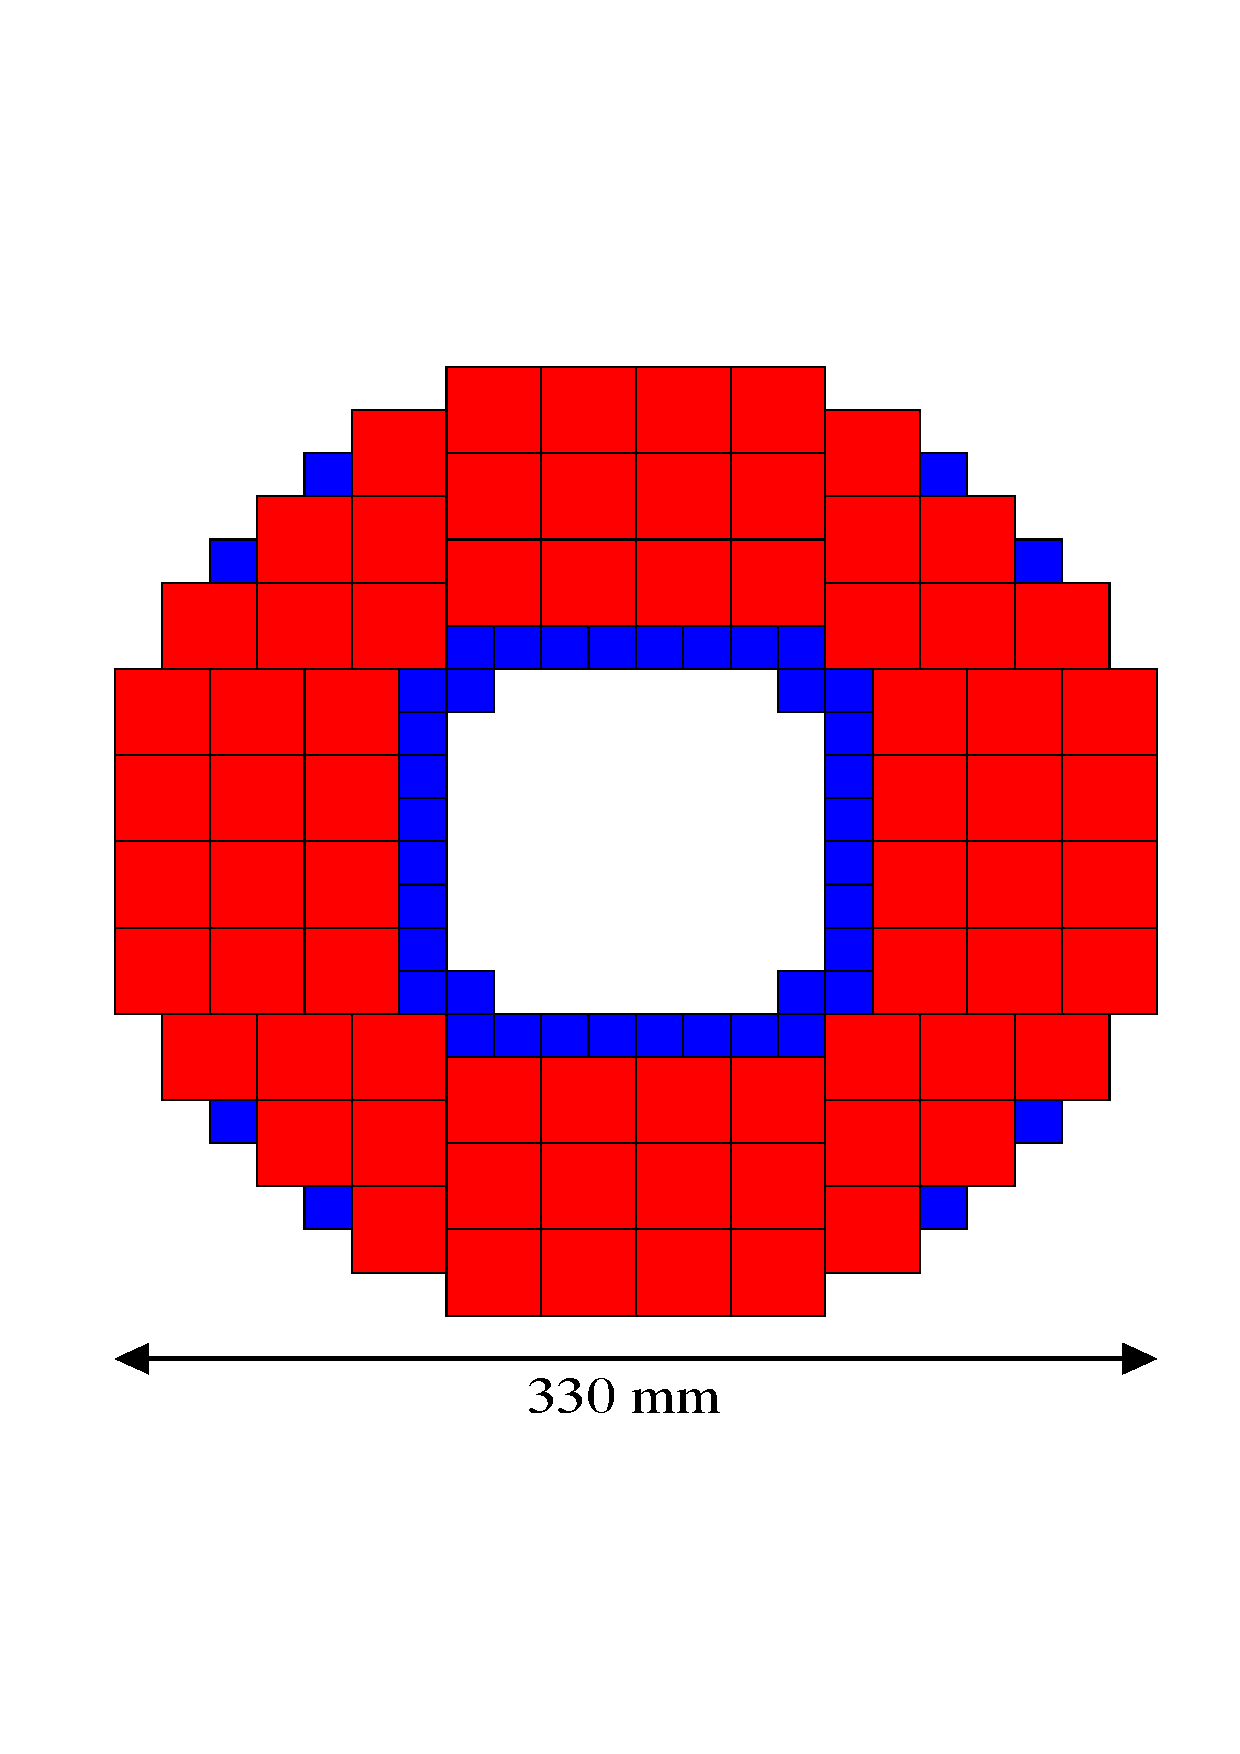
\includegraphics[width=0.85\columnwidth]{./fig/FTHodoLayout.pdf} 
\caption{The arrangement of plastic scintillator tiles in the FT-Hodo. The blue (red) squares represent the $15\times 15$~mm ($30\times 30$~mm) tiles afor each layer. } 
\label{Fig:FTHodoLayout} 
\end{figure}
The upstream and downstream layers utilize 7~mm and 15~mm thick scintillator tiles, respectively. The upstream (thin) layer is employed to reduce photon conversion in the FT-Hodo, while the thicker layer provides the signal with the most accurate timing information for the event. To increase the number of scintillation photons collected from each tile, four WLS fibers were embedded in the P30 tiles and 2 in the P15 tiles. In addition, the WLS fibers were glued with Bocron BC600 glue (CHECK Epotek 301-2) inside diagonal holes that maximizes the path length in the scintillator and allows for the tiles to be arranged without any dead space between the elements. Each tile was polished and painted with two layers of Bicron BC620 reflective paint for the sides and 3 layers for the scintillator faces and secured in position on the surface of a 2~mm thick plastic support board. There is a 9~mm clearance for each layer for routing the optical fibres to the readout electronics through a $\Delta$-shaped sheathing on the bottom end of the FT-Hodo. The front and back faces are covered by lightproof carbon fiber material that is screwed on supporting structures made out of hexagonal plastic spacers (15~mm wide ans 22 or 15 ~mm tall depending on the layer). This results in a total detector thickness of 44~mm. A 1~mm thick plastic strip traces the outer contour of the FT-Hodo and is glued on the spacer supports. Figure~\ref{Fig:CADFT-Hodo} shows a CAD drawing of the FT-Hodo showing half of one layer of tiles, the location of the plastic supports for the light proofing structure and the plastic strip.  
\begin{figure}[th!]
\centering 
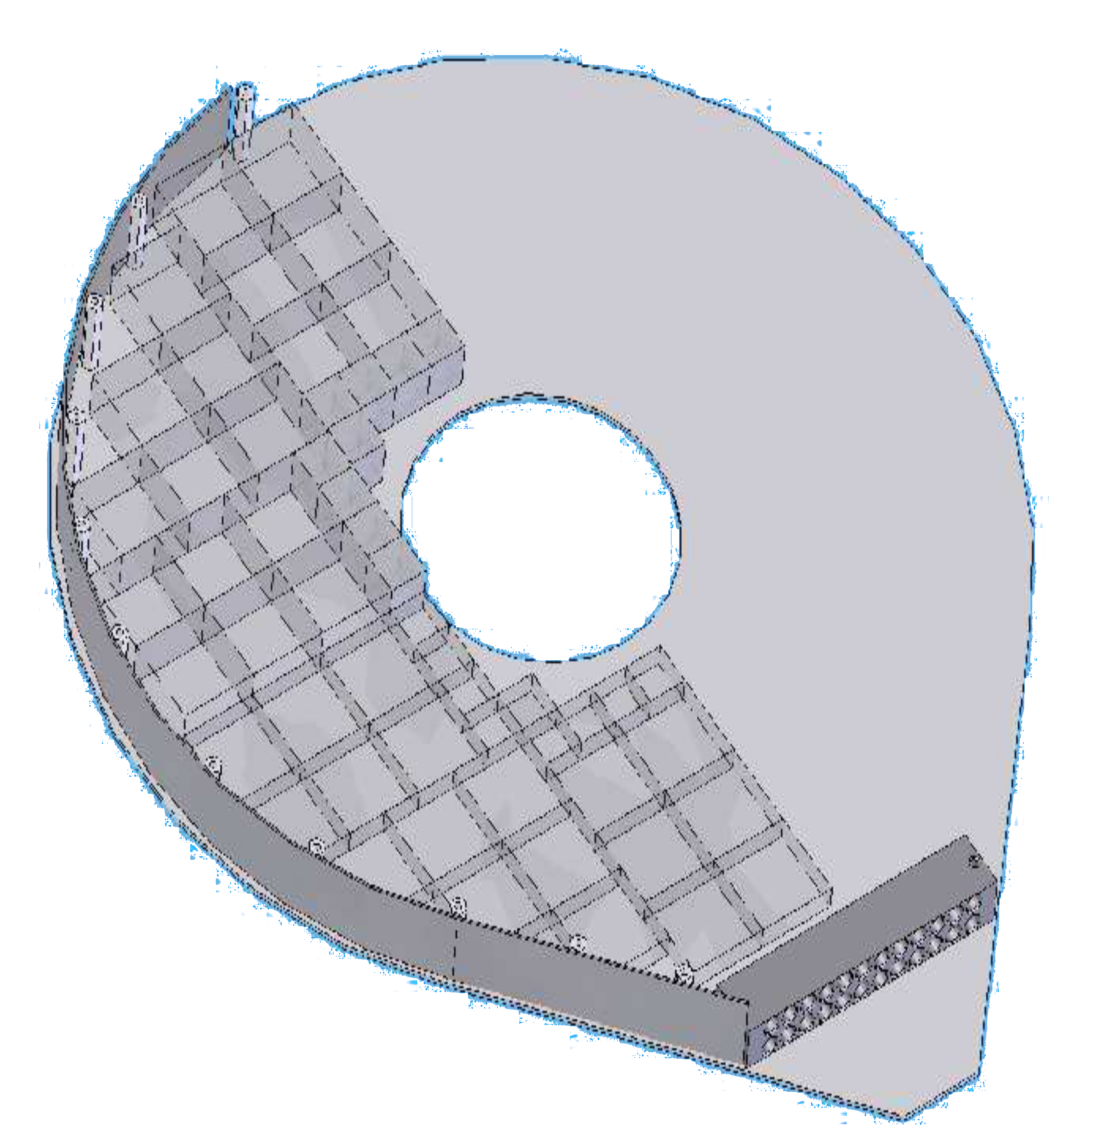
\includegraphics[width=0.85\columnwidth]{./fig/CADFT-Hodo.pdf} 
\caption{CAD drawing of the FT-Hodo showing half of layer 1, the location of the plastic spacers, and the plastic strip that traces the outer contour. } 
\label{Fig:CADFT-Hodo} 
\end{figure}

With the typical maximum doses determined through GEANT4 simulations with realistic beam and target parameters and without the shielding effects of the Moeller cone (see \ref{sec:integration}, the FT-Hodo will experience a light loss of 20\% in the WLS fibre ~\cite{TDR42} after 3.5 years, whereas the plastic scintillators will experience a lightloss of 20\% after 300 years~\cite{TDR41}. Both scintillators and fibers also show natural annealing processes, which can effectively compensate for the radiation damage~\cite{TDR43}.  

The analog signal from the SiPM is fed directly to a custom designed pre-amplifier board designed by the INFN-Genova electronics group. The boards host 8 independent channels each coupled to a SiPM and are mounted in pairs in the slots of a custom crate, mechanically compatible with the VME standard. The 16 SiPMs connected to each pair of boards are mounted on a mezzanine PCB, which distribute the bias HV to each SiPM and collects their signals for the amplifier inputs. The schematic of one channel of the SiPM amplifier board, excluding the HV bias network is shown in Fig.~\ref{Fig:FTHODOAmpBoard}  
\begin{figure}[th!]
\centering 
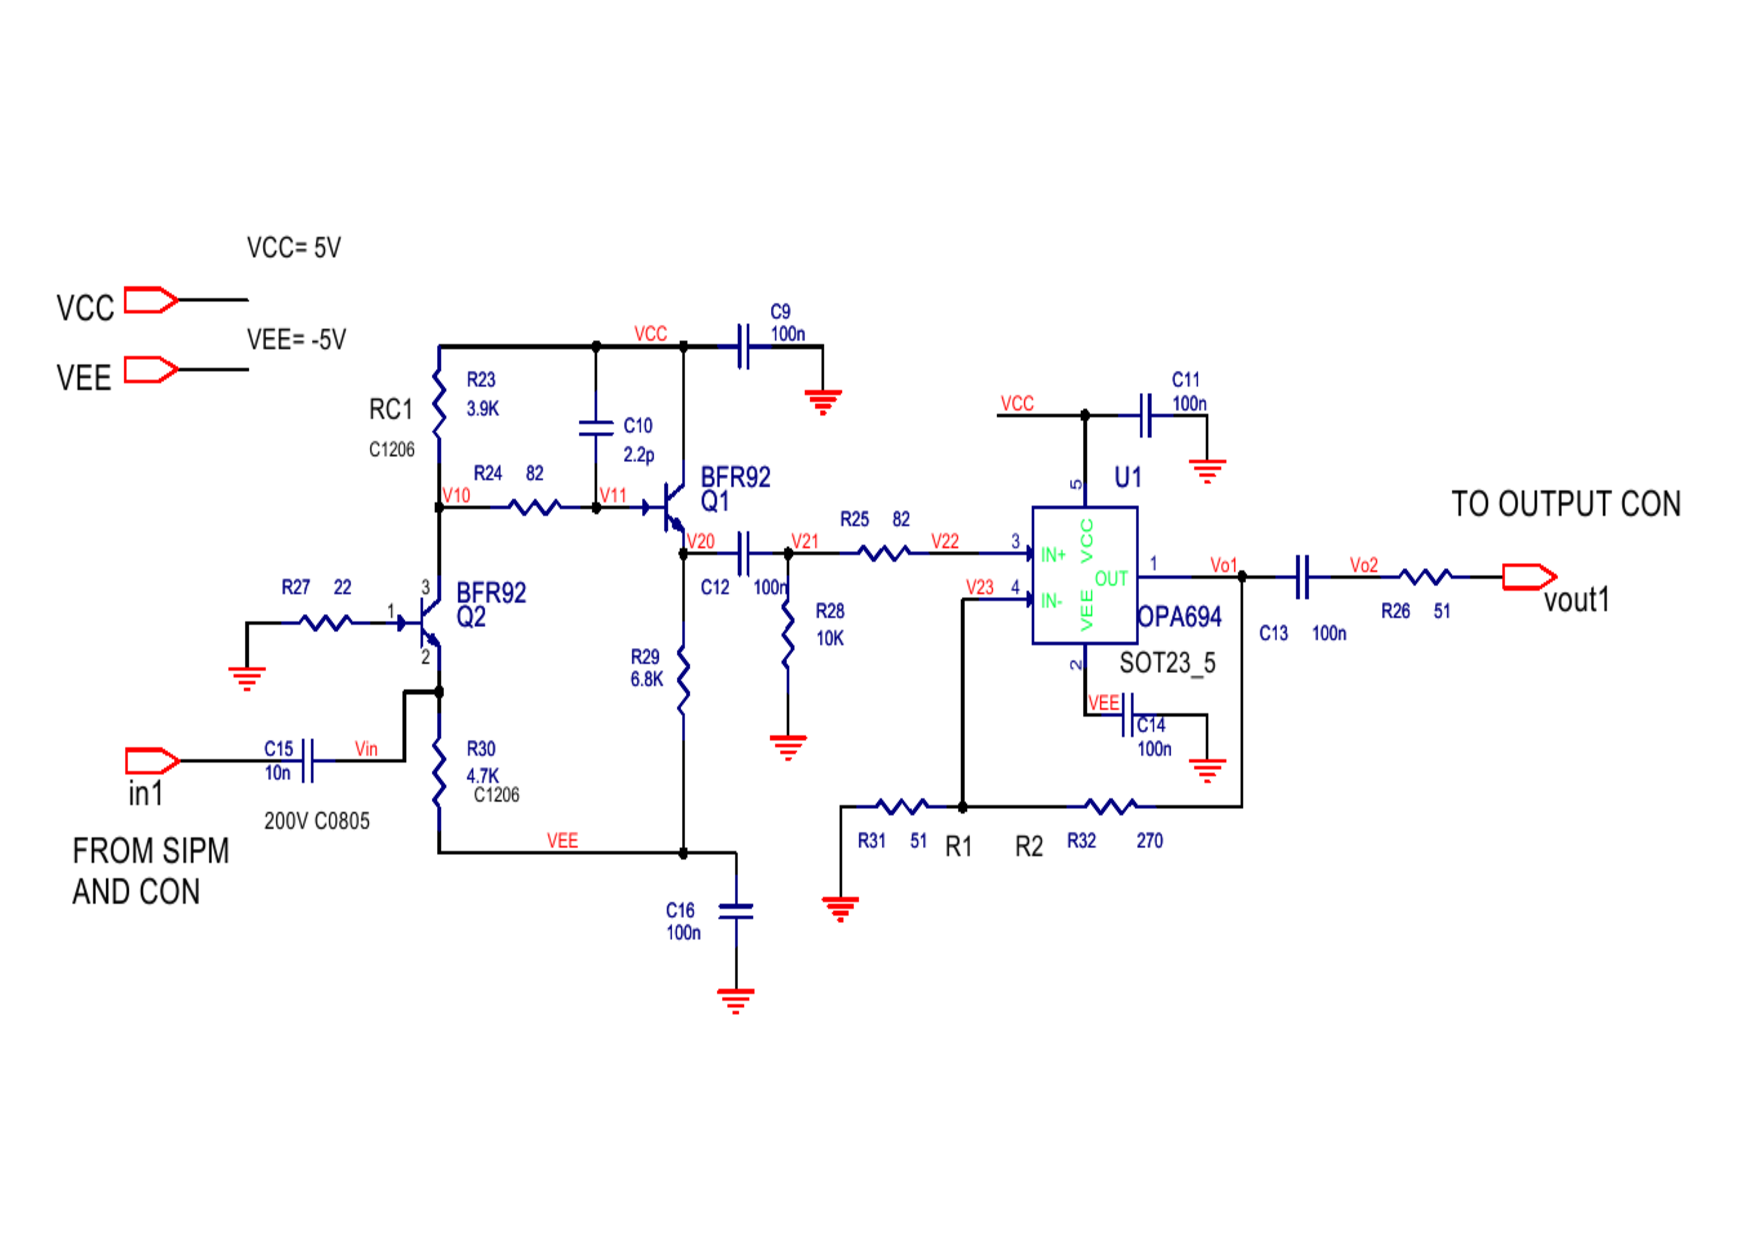
\includegraphics[width=0.95\columnwidth]{./fig/FTHODOAmpBoard.pdf} 
\caption{NEED TO Check if UP2Date: Schematic of a single channel of the amplifier board for SiPM.} 
\label{Fig:FTHODOAmpBoard} 
\end{figure}
The first stage is based on a Bipolar Junction NPN transistor in a common base configuration, while the second is composed by a OPA694 operational amplifier in a non-inverting configuration. The two BRF92 transistors have been chosen since they are low noise transistors with a high cut-off frequency and good stability. The two stages are coupled together with a 100~nF capacitor to remove the DC component of the signal from the second transistor. The amplifier is coupled to the output connector through a 100~nF capacitor and a 50~$\Omega$ resistor to remove any DC component from the last stage and match the impedance of the output cable. 


The signal from each SiPM after amplification is continuously digitized by the JLab fADC 250 boards and, if the trigger condition is satisfied, samples are stored for further analysis. The data acquisition and slow controls system for the FTHodo are similar to the FTCal and we refer to that for more details. The SiPMs operate with a bias voltage of 50-55.5~V, which is provided by three CAEN A1737P HV boards. 30 independent HV channels are used to operate each SIPM board hosting 8 sensors. These groups of 8 SIPMs were selected according to their gain. The low voltage system used for the FTHodo is the same as the one used for FTCal.


\subsection{The MicroMegas tracker (FT-Trck)}
For a precise determination of the scattered electron angle, a tracker complements the FT-Cal and FT-Hodo detectors. The FT-Trck uses the same technology adopted by the CLAS12 central and forward Micromegas detectors. We refer to \cite{mm} for a detailed description of  these devices. In this section we just describe the specific design of the FT-Trck.
\begin{figure}[th!]
\centering 
\includegraphics[width=1.0\columnwidth]{./fig/FTtrck.eps}
\caption{3D view of the tracker equipped with front-end electronics.}
\label{fig:ft-trck} 
\end{figure}

Two double-layers of Micromegas detectors
are located in front of the hodoscope, in the space between the FT
and the High Threshold Cerenkov Counter
(HTCC). Two detectors are indeed a good compromise
to achieve an efficient background rejection
and track reconstruction with a low
material budget. Each layer is
composed by a double faced Micromegas disk
bulked on a common PCB. Each side of the
PCB displays strips, the downstream ones being
perpendicularly oriented to the upstream
ones. This particular geometry enables the
determination of the (X,Y) coordinates of a
track. To limit the number of electronic channels
the pitch chosen was 500 $\mu$m, which leads
to a resolution better than than 500/$sqrt(12)\sim 150$ $\mu$m.
A drift space of 5 mm together with an amplification gap of 128  $\mu$m provide
a good efficiency.
The two double-layers, centered on the beam axes,   cover polar angles from 2.5$^o$ to 4.5$^o$ with an active area defined
between 70 mm inner radius and a 143 mm outer radius.
The total number of channel is 3072.
Figure~\ref{fig:ft-trck} shows the CAD implementation of the detector. 
the FT-Trck readout uses the same DAQ scheme adopted for the CLAS12 Central Micromegas. It  consists
of a Front-End (FE) and a  Back-End (BE) unit. 

The FE
electronic is responsible for signal pre-amplification, shaping,  buffering during the trigger generation
process, data digitization and compression.
Due to the limited space available, the FE electronic 
is designed to be placed off-detector.
The micro-coaxial cable assemblies
connect the detectors and the FE boards. Non-amplified
analog signals transit via the cable
assemblies from the chambers to the FE electronics.
The 512-channel FE Units (FEU)
 are housed in 4U crates attached to the FT-Cal mechanical supports and  located
in the shadow of the CLAS12 torus coils.

The  BE electronic is
responsible for data concentration providing the 
interface to ClAS12
event building system. It is the same used for the Central Micromegas. Details are available in Ref.~\cite{mm}.

Each Micromegas layer  is powered with 
 450 V for the micro-mesh,
and 1000 V for the drift electrode.
The FT-Trck FE power supply is located 12 m away from the crates. The 15 W power produced by each crate is dissipated  by compressed air. An interlock system between the cooling
infrastructure and the low voltage power supply
prevents powering the FE crates
when cooling is off. 

The gas used 
is a mixture of Argon, isobutane (up to
10$\%$) and CF4 (up to 5$\%$). The use of
CF4 ensures a good time resolution (around
10-15 ns). The gas distribution is the same of the one used by the Central Micromegas system.


